\documentclass[../DS04.tex]{subfiles}
\graphicspath{{./figures/}}

% \subimport{/home/nora/Documents/Enseignement/Prepa/bpep/exercices/DS/cinetique_methylhydrazine/}{sujet.tex}

\begin{document}

\begin{pycode}
import numpy as np
MH = 5    # mol.L^-1
t12 = 62.5   # min
ko0 = 1/(2*t12)
ko1 = np.log(2)/(t12*MH)
ko2 = 1/(t12*MH**2)

R = 8.31

k1 = ko1
k2 = 2.62e-3
lnkk = np.log(k2/k1)

T1 = 298 # K
T2 = 313 # K
TT = T1*T2/(T1-T2)

Ea = -R*TT*lnkk

\end{pycode}

\exercice[26]{\'Etude cinétique de l'oxydation de la méthylhydrazine}
\enonce{
	L’hydrazine, de formule \ce{N2H4}, est, à température ambiante, un liquide
	incolore cancérogène et toxique pour les organismes aquatiques mais qui ne
	répond pas aux critères environnementaux de persistance et de bioaccumulation.
	Son odeur est comparable à celle de l'ammoniac. L'hydrazine est un composé
	inflammable, extrêmement corrosif et irritant. L'hydrazine est principalement
	utilisée sous forme d'hydrate de formule \ce{N2H4},\ce{H2O}. L'hydrate
	d'hydrazine a été synthétisé pour la première fois en 1889 par Theodor
	Curtius, un chimiste allemand. Actuellement, sa production mondiale annuelle
	est estimée à plus de \SI{50 000}{tonnes}.

	Le secteur de l’aérospatial est le plus gros consommateur d’hydrazine pure.
	En effet, si dès la fin de la seconde guerre mondiale, l'hydrate d'hydrazine
	a été utilisé comme carburant dans le premier avion de chasse à réaction,
	l’hydrazine pure et ses dérivés méthylés sont utilisés depuis plus de 50 ans
	comme propergol en association avec le tétraoxyde de diazote \ce{N2O4} dans
	les fusées (notamment Ariane) ou monergol pour la mise en orbite des
	satellites et sondes spatiales.

	La méthylhydrazine \ce{(H3C)HN-NH2} est également utilisée comme biergol en
	association avec un oxydant fort tel que le tétraoxyde de diazote (\ce{N2O4}).

	\textbf{On s’intéresse ici à l’oxydation de la méthylhydrazine,} notée par
	la suite MH, par le dioxygène dissous en milieu strictement monophasique
	modélisée par l’équation de réaction~:
	\[
		\ce{2(H3C)HN-NH2(aq) + 1O2(aq) -> }
		{\text{produits d'oxydation}}
	\]
	\begin{tcb}(odgr){Aide au calcul}
		\begin{gather*}
      \frac{1}{\py{2}\times\py{t12}} = \py{fr'\num{{{ko0:.2e}}}'}
			\quad ; \quad
      \frac{\ln 2}{\py{t12}\times\py{MH}} = \py{fr'\num{{{ko1:.2e}}}'}
			\quad ; \quad
      \frac{1}{\py{MH}^{2}\times\py{t12}} = \py{fr'\num{{{ko2:.2e}}}'}
      \\
      ~
      \\
      \frac{\py{T1}\times\py{T2}}{\py{T1}-\py{T2}} = \py{fr'\num{{{TT:.1f}}}'}
      \quad ; \quad 
      \ln \frac{\py{fr'\num{{{k2*1e3:.2e}}}'}}{\py{fr'\num{{{k1*1e3:.2e}}}'}} =
      \py{fr'\num{{{lnkk:.2e}}}'}
      \quad ; \quad 
      \num{8.31}\times \py{fr'\num{{{-TT:.2e}}}'} \times \py{fr'\num{{{lnkk:.2e}}}'}
      = \py{fr'\num{{{Ea:.2e}}}'}
		\end{gather*}
	\end{tcb}
}

%%%%%%%%%%%%%%%%%%%%%%%%%%%%%%%%%

\QR[2]{%
	Donner deux définitions de la vitesse de la réaction, l'une avec \ce{[MH]} et
	l'autre avec \ce{[O2]}.
}{%
	\[
		\boxed{v(t)=-\dfrac{1}{2}\dv{[\ce{MH}]}{t}=-\dfrac{1}{1}\dv{[\ce{O2}]}{t}}
	\]
}

%%%%%%%%%%%%%%%%%%%%%%%%%%%%%%%%%

\enonce{
	Quatre séries de mesures sont réalisées à \SI{298}{K} en faisant varier la
	concentration initiale en \ce{O2}, la concentration initiale en MH étant
	fixée à $\SI{5.00e-3}{mol.L^{-1}}$. Dans le tableau suivant, sont reportées
	les valeurs de la variation $v_0 = -\dv{[\ce{O2}]}{t}\/(t=0)$ et le
	temps de demi-réaction $t_{1/2}$.

	\begin{center}
		\begin{tabularx}{.7\linewidth}{*{4}{Y}}
			\toprule
			$[\ce{O2}]_0$ ($\SI{e-4}{mol.L^{-1}}$)                 &
			$[\ce{MH}]_0$ ($\SI{e-3}{mol.L^{-1}}$)                 &
			$v_0$ ($\SI{e-6}{mol.L^{-1}.min^{-1}}$) &
			$t_{1/2}$ (\si{min})
			\\
			\midrule
			0,25                                                   &
			5,00                                                   &
			0,29                                                   &
			60,0
			\\
			1,07                                                   &
			5,00                                                   &
			1,11                                                   &
			65,0
			\\
			1,78                                                   &
			5,00                                                   &
			2,27                                                   &
			62,0
			\\
			3,02                                                   &
			5,00                                                   &
			3,32                                                   &
			63,0
			\\
			\bottomrule
		\end{tabularx}
	\end{center}
}

\QR[1]{%
La réaction est supposée admettre un ordre. La constante de vitesse est notée
$k$ et les ordres partiels par rapport à la méthylhydrazine et au dioxygène
sont notés respectivement $p$ et $q$. Exprimer la vitesse de réaction à l’aide
de ces paramètres.
}{%
\[
	\boxed{v(t)=k[\ce{MH}]^p(t)\times [\ce{O2}]^q(t)}
\]
}

\QR[6]{%
	Expliquer en quoi consiste la méthode de dégénérescence de l’ordre. Est-ce
	qu'on peut dire que les concentrations initiales en MH et \ce{O2} sont en
	accord avec cette méthode ? Si oui, donner une expression approchée de la
	vitesse de réaction.
}{%
	La méthode de la dégénérescence de l'ordre consiste à introduire en excès tous
	les réactifs sauf un. Alors on peut considérer que la concentration des
	réactifs en excès ne varie presque pas au cours du temps, et donc que seule la
	concentration du réactif \ce{A} introduit en faible proportion influe sur la
	vitesse de la réaction qui peut se mettre sous la forme
	\[
		v(t)=k\ind{app}[\ce{A}]^{\alpha}(t)
	\]
	avec $k\ind{app}$ la constante de vitesse apparente. Cette méthode permet
	d'avoir accès à l'ordre partiel sur le réactif \ce{A}.

	La concentration en MH est au moins 10 fois supérieure à celle en \ce{O2},
	donc c'est en accord avec la méthode de la dégénérescence de l'ordre. On peut
	alors donner une expression approchée de la vitesse de réaction
	\[
		\boxed{
			v(t)\approx
			k[\ce{MH}]_0^p\times [\ce{O2}]^q(t) =
			k\ind{app} [\ce{O2}]^q(t)
			\qavec
			k\ind{app}= k[\ce{MH}]_0^p
		}
	\]
}

\QR[4]{%
	Définir ce qu'est la méthode différentielle. Pour cette réaction admettant un
	ordre, comment peut-on employer cette méthode afin de déterminer la valeur de
	l'ordre partiel $q$ par rapport au dioxygène~?
	À l'aide de la Figure~\ref{fig:lnv}, déterminer alors la valeur de $q$.
	\begin{figure}[htbp!]
		\centering
		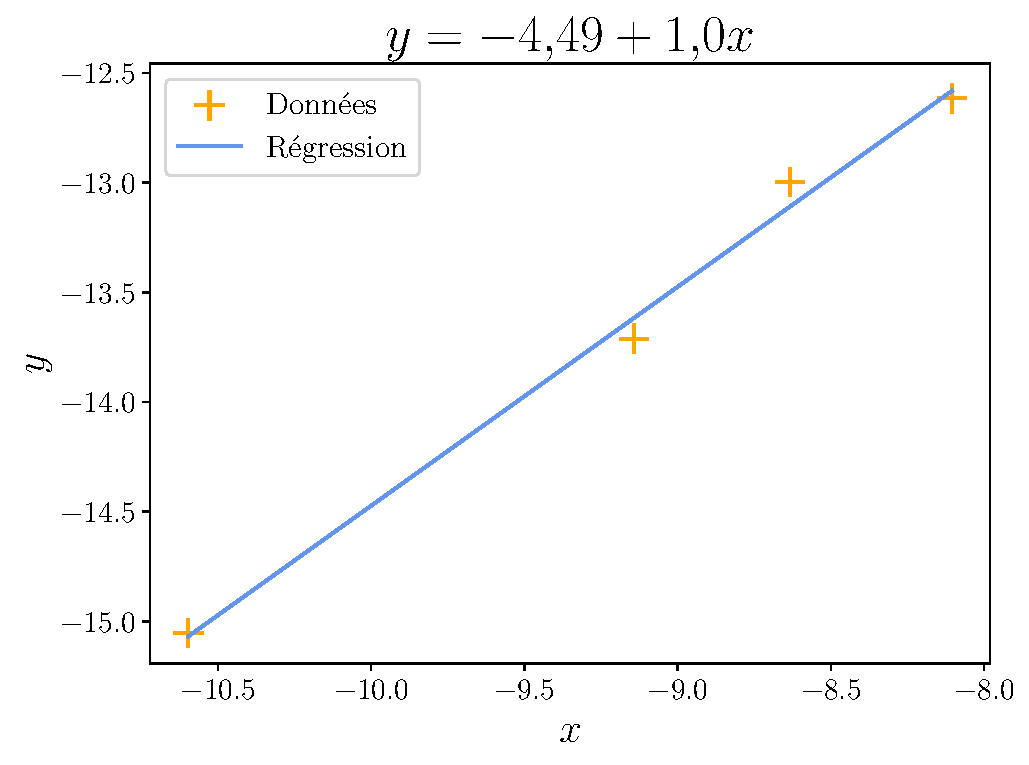
\includegraphics[width=.5\linewidth]{trace_lnv}
		\caption{Régression linéaire}
		\label{fig:lnv}
	\end{figure}
}{%
	La méthode différentielle consiste à travailler directement avec la vitesse,
	en traçant $v$ connaissant les concentrations en réactifs. Dans notre cas,
	la vitesse initiale peut s'écrire~:
	\[
		v_0=k\ind{app}[\ce{O2}]_0^q
		\qsoit
		\ln(v_0)=\ln(k\ind{app})+q\ln\pa{[\ce{O2}]_0}
		\qavec v_0=-\dv{[\ce{O2}]}{t}\/(t=0)
	\]
	Ainsi, on trace
	\[
		y\tikzmark{yn} = a\tikzmark{an}x\tikzmark{xn} + b\tikzmark{bn}
	\]
	\tikz[remember picture, overlay]
	\draw[-stealth, transform canvas={xshift=-6pt, yshift=-6pt}]
	(pic cs:yn) --++ (-10pt,-10pt)
	node[anchor=north east] {$\ln(v_0)$}
	;
	\tikz[remember picture, overlay]
	\draw[-stealth, transform canvas={xshift=-5pt, yshift=-6pt}]
	(pic cs:an) --++(-10pt,-10pt)
	node[anchor=north east] {$q$}
	;
	\tikz[remember picture, overlay]
	\draw[-stealth, transform canvas={xshift=0pt, yshift=-6pt}]
	(pic cs:xn) --++(5pt,-10pt)
	node[anchor=north] {$\ln ([\ce{O2}]0)$}
	;
	\tikz[remember picture, overlay]
	\draw[-stealth, transform canvas={xshift=3pt, yshift=-6pt}]
	(pic cs:bn) --++(10pt,-10pt)
	node[anchor=north west] {$\ln (k\ind{app})$}
	;
	\vspace{+15pt}

	On constate que l'ajustement affine passe bien par les points. On en déduit
	$\boxed{q=1}$.
}

\QR[5]{%
En supposant que la valeur de cet ordre initial n'est pas modifiée au cours du
temps, établir l'expression du temps de demi-réaction $t_{1/2}$ en fonction
d'une constante apparente $k\ind{app}$ à définir. Comparer aux données
expérimentales et conclure quant à la validité de cette hypothèse.
}{%
On supposant $q=1$ pour tout temps, et dans le cas de la méthode de la
dégénérescence de l'ordre, on peut écrire
\[
	v(t)=k\ind{app}[\ce{O2}](t)
	\qavec
	v(t)=-\dv{[\ce{O2}]}{t}
\]
Par intégration, on obtient
\[
	[\ce{O2}](t)=[\ce{O2}]_0\exp\pa{-k\ind{app}t}
\]
Par définition du temps de demi-réaction,
\[
	[\ce{O2}](t_{1/2})=\dfrac{[\ce{O2}]_0}{2}
	\qsoit
	\boxed{t_{1/2}=\dfrac{\ln(2)}{k\ind{app}}}
\]
On en déduit que $t_{1/2}$ est indépendant de la concentration initiale
$[\ce{O2}]_0$, ce qui est en accord avec des données expérimentales. On en
conclut que la valeur de l'ordre initial n'est pas modifiée au cours du temps.
}

\enonce{
	Des mesures complémentaires ont permis de mesurer un ordre partiel égal à 1
	par rapport à la méthylhydrazine.
}

\QR[4]{%
En considérant $t_{1/2} = \SI{62.5}{min}$, déterminer la valeur de la constante de vitesse à
\SI{298}{K}, en $\si{L.mol^{-1}.min^{-1}}$.
}{%
On prend la valeur moyenne $t_{1/2}=\SI{62.5}{min}$, et on en déduit
\[
	k\ind{app}=\dfrac{\ln(2)}{t_{1/2}}
	\qavec
	k\ind{app}=k[\ce{MH}]_0
	\qdonc
	\boxed{k=\dfrac{\ln(2)}{t_{1/2}[\ce{MH}]}=\SI{2.22}{L.mol^{-1}.min^{-1}}}
\]
}

\QR[4]{%
À \SI{313}{K}, la détermination expérimentale de la constante de vitesse
conduit à une valeur de $\SI{2,62}{L.mol^{-1}.min^{-1}}$. Calculer la valeur de
l'énergie d'activation de la réaction d'oxydation de la méthylhydrazine par le
dioxygène en supposant que cette grandeur est indépendante de la température.
On prendra $R=\SI{8.31}{J.K^{-1}.mol^{-1}}$.
}{%
D'après la loi d'Arrhénius,
\[
	k(T)=A\exp\pa{-\dfrac{E_A}{RT}}
\]
En notant $k_1=k(T_1)$ et $k_2=k(T_2)$, on a
\begin{gather*}
		\frac{k_1}{k_2}
		= \frac{A \exp \left( - \dfrac{E_a}{RT_1} \right)}{A
			\exp \left( - \dfrac{E_a}{RT_2} \right)}
		= \exp \left( \frac{E_a}{R} \left(
			\frac{1}{T_2} - \frac{1}{T_1} \right) \right)
		\\\Lra
		\boxed{E_a = R \frac{T_1T_2}{T_1-T_2}\ln \left( \frac{k_1}{k_2} \right)}
    \qav
    \left\{
    \begin{array}{rcl}
      R & = & \SI{8.31}{J.K^{-1}.mol^{-1}}
      \\
      T_1 & = & \SI{298}{K}
      \\
      T_2 & = & \SI{313}{K}
      \\
      k_1 & = & \SI{2.22}{L.mol^{-1}.min^{-1}}
      \\
      k_2 & = & \SI{2.62}{L.mol^{-1}.min^{-1}}
    \end{array}
    \right.\\
    \AN
    \xul{
      E_a = \py{fr'\SI{{{Ea*1e-3:.2e}}}{{kJ.mol^{{-1}}}}'}
    }
\end{gather*}
}

\end{document}
